\usetikzlibrary{calc,decorations.pathmorphing,shapes.geometric}
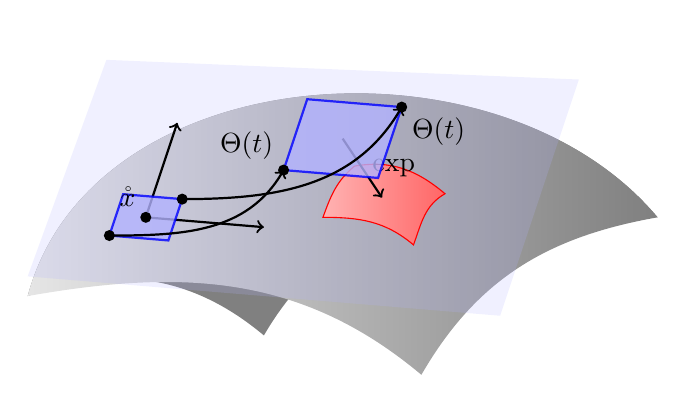
\begin{tikzpicture}[thick,scale=1, every node/.style={scale=1}]
    \draw[fill=black!50, draw=none]
      (0, 0) to[out=20, in=140] (3, -0.5) to [out=60, in=160]
      (8, 1) to[out=130, in=75] cycle;
    
    \shade[thin, left color=black!10, right color=black!50, draw=none]
      (0, 0) to[out=10, in=140] (5, -1) to [out=60, in=190] 
      (8, 1) to[out=130, in=75] cycle;

    \coordinate (g) at (1.5,1) ;

    % Tangent space at g
    \fill[fill=blue!30,opacity=.2] (0,0.25) -- (6,-0.25) -- (7,2.75) -- (1,3) -- cycle;
    % \node[rotate=0] at (1.75,2.5) {$T_{\mathring{x}}\mathcal{X}\simeq\mathfrak{x}$};
    \draw[->] (g) -- ++(1.5,-0.125);
    \draw[->] (g) -- ++(0.4, 1.2);

    % Initial tangent interval
    \coordinate (DX0) at ($0.125*(6, -0.5)$);
    \coordinate (DY0) at ($0.175*(1, 3)$);
    \coordinate (ulT0) at ($(g) - 0.5*(DX0) - 0.5*(DY0)$) ;
    \coordinate (olT0) at ($(ulT0) + (DX0) + (DY0)$) ;
    \fill[draw=blue,fill=blue!30,opacity=.8] (ulT0) -- ++(DX0) -- ++(DY0) -- ++($-1*(DX0)$) -- cycle;
    % \fill (ulT0) circle (2pt) node[below left] {$\ul\Theta_0$};
    % \fill (olT0) circle (2pt) node[above right] {$\ol\Theta_0$};
    \fill (ulT0) circle (2pt) ;
    \fill (olT0) circle (2pt) ;

    %% Final tangent interval
    \coordinate (TT) at (4,2);
    \coordinate (DXT) at ($0.2*(6, -0.5)$);
    \coordinate (DYT) at ($0.3*(1, 3)$);
    \coordinate (ulTT) at ($(TT) - 0.5*(DXT) - 0.5*(DYT)$) ;
    \coordinate (olTT) at ($(ulTT) + (DXT) + (DYT)$) ;
    \coordinate (gT) at (4.5,1.25) ;
    
    % Exponentiated
    \shade[thin, left color=red!30, right color=red!60, draw=red]
      ($(gT)+(-0.75,-0.25)$) to[out=0, in=140] ($(gT)+(0.4,-0.6)$) to [out=70, in=-150] 
      ($(gT)+(0.8,0.05)$) to[out=140, in=10] ($(gT)+(-0.35,0.4)$)
      to[out=-140, in=70]  cycle;
    
    % Exponential arrow
    \draw[->,thick] (TT) -- (gT) node[midway, right] {$\exp$};
    
    \fill[draw=blue,fill=blue!30,opacity=.8] (ulTT) -- ++(DXT) -- ++(DYT) -- ++($-1*(DXT)$) -- cycle;
    \fill (ulTT) circle (2pt) node[above left] {$\ul\Theta(t)$};
    \fill (olTT) circle (2pt) node[below right] {$\ol\Theta(t)$};
    % \fill (ulTT) circle (2pt) ;
    % \fill (olTT) circle (2pt) ;

    % Trajectory from ulT0 to ulTT
    \draw[->,thick] (ulT0) to[out=0, in=-120] (ulTT);
    \draw[->,thick] (olT0) to[out=0, in=-120] (olTT);
    
    % Points at g 
    \fill (g) circle (2pt) node[above left] {$\mathring{x}$};
    % \fill (gT) circle (2pt) node[below right] {$\mathring{x}_{t+\Delta t}$};
    \node at (7.5, 0.5) {$\calX$} ;

\end{tikzpicture}